\chapter{Mathematical Modelling of Nucleotide Excision Repair (NER)}
\pagestyle{plain}
%%\documentclass[a4paper, 12pt]{article}
%%\usepackage[english]{babel}
%%\usepackage{graphicx}
%%\makeatletter
%%\def\ScaleIfNeeded{%
%%	\ifdim\Gin@nat@width>\linewidth
%%		\linewidth
%%	\else
%%		\Gin@nat@width
%%	\fi
%%}
%%\makeatother
%%\def\TCop{\textsuperscript{\textcopyright}}
%%\def\TReg{\textsuperscript{\textregistered}}
%%\def\TTra{\textsuperscript{\texttrademark}}
%%\usepackage[applemac]{inputenc}
%%\usepackage{color}
%%\usepackage{cite}
%%\pagestyle{headings}
%
%%\newpage
%%\usepackage[T1]{fontenc}
%%\newcommand{\changefont}[3]{
%%\fontfamily{#1} \fontseries{#2} \fontshape{#3} \selectfont}
%%\changefont{phv}{m}{n}
%%\begin{document}
%\section{Introduction}
An essential advantage for the research on Nucleotide Excision Repair (NER) is the ability to inflict UV-induced DNA damages within a locally confined area in the cell nucleus \cite{Mone2001}. This technique reformed the investigation of chromatin associated processes whose \textit{in vivo} analysis was, until then, focusing on enzyme mobility and exchange dynamics at steady state performed with photobleaching experiments \cite{Houtsmuller2001,Mone2004}. In contrast, the enclosed distribution of single stranded DNA damages causes the local activation of a multi-protein repair machinery which in turn allows to study the \textit{de novo} assembly and dissociation kinetics of single repair factors. Exploiting this standard experimental setup we acquired a comprehensive data set comprising the accumulation and dissociation time series of seven individual repair enzymes. In addition, we were able to directly quantify newly synthesized DNA measuring the incorporation of a fluorescently modified nucleotide analogue.\\
Based on this data we developed a mathematical model that is able to explain the connection between the dynamic exchange of individual repair factors at the chromatin on one hand and the overall time scale of the repair process on the other. The exact parametrization of the model was adapted iteratively in correspondence with a profile likelihood estimation leading to identifiable parameters and hence an increased predictive power of the model. As a consequence our model can reliably predict the behaviour of an experimentally not accessible DNA intermediate within the repair process.\\
   
The experiments reported in this chapter were planed and conducted by Martijn Luijsterburg (accumulation and FLIP experiments) and Paul Verbruggen (EdU incorporation).
	
	
\section{Fluorescent time-laps imaging of the NER process}

\subsection{Locally inflicted UV-induced DNA damage}
\label{sec:local_irradiation}
\begin{figure}[htbp]
	\begin{center}
		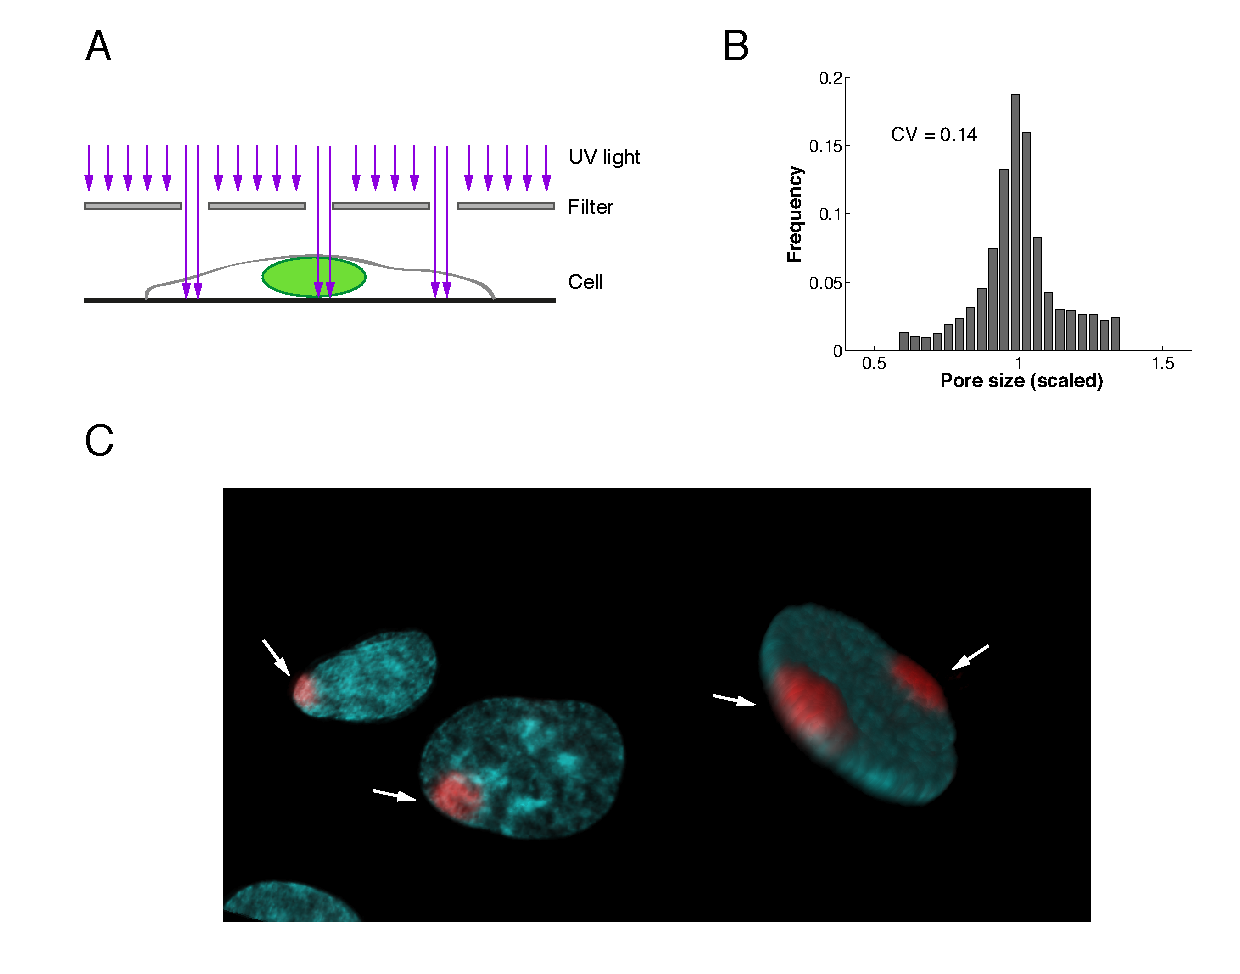
\includegraphics[width=1\textwidth]{Abbildungen/figure2_1.pdf}
		\caption{\textbf{Local irradiation leads to spatially confined DNA damage.} A) Schematic illustration of the experimental setup. UV-light (purple arrows) is transmitted through a UV filter containing pores with 5 \textmu m diameter. Local irradiation of the chromatin occurs, if a pore is located above a cell nucleus. (\textbf{reprint of }) B) Distribution of the pore sizes within the UV irradiation mask (n=5008) - \textbf{ask paul how he did it} C) Partially UV-irradiated nuclei of cultivated mammalian cells were made visible with a blue-fluorescent DNA stain. Red fluorescence depicts incorporation of nucleotides due to Nucleotide Excision Repair of damaged DNA.}
		\label{fig:accuMethod}
	\end{center}
\end{figure} 

To observe the dynamic behavior of NER factors upon local infliction of DNA damage we applied the experimental setup developed by Mon\'e \textit{et al.} (2001)\cite{Mone2001}. Therein, NER competent cells are covered with a polycarbonate UV filter containing pores with a given diameter (cf.\ Figure \ref{fig:accuMethod}A). For our purposes cells were grown on uncoated 24 mm coverslips before overlaid with a mask including pores with 5 \textmu m diameter \cite{Verbruggen2014}. Figure \ref{fig:accuMethod}B illustrates the realistic deviation of pore diameters due to manufacturing inaccuracies. The actual size distribution has a very small CV of 0.14 indicating a negligible effect on the filter's transmissivity. Filter-covered cells were immediately irradiated with a dose of 100 $\text{J/m}^\text{2}$ of UV-C with a fluency of 3.85 $\text{W/m}^\text{2}$. Due to the specific pore density (4 x $\text{10}^\text{5}$ pores/$\text{cm}^\text{2}$) we could observe nuclei containing either one damage spot or no spot at all. Very rarely two spots per cell were present (cf.\ Figure \ref{fig:accuMethod}C, white arrows indicate damage spot). Consequently, with this technique one can measure NER in damaged nuclei as well as undamaged control nuclei in the same experiment.



\subsection{Repair factor accumulation and dissociation occur on different time scales}
\label{subsec:AccuFlipExp}
The ability to locally inflict DNA damage with a discrete dose of UV-C allows to study the accumulation and exchange behavior of fluorescently tagged repair proteins under different experimental conditions. In the following we describe the comprehensive dataset acquired by Luijsterburg \textit{et al.} (2010)\cite{Luijsterburg2010}, which represents the basis of our quantitative analysis of the NER process. In total, the kinetics of seven repair factors were measured: i) XPC, the lesion recognition factor; ii) TFIIH, the helicase responsible for DNA unwinding; iii) XPA and RPA, which bind and thereby protect single stranded DNA against cleavage iv) the exonucleases XPF/ERCC1 and XPG performing the incision of the damaged DNA strand and v) PCNA, which loads the DNA polymerase and hence indirectly provides insight into the DNA repair-synthesis kinetic. \\
\begin{figure}[htbp]
\begin{center}
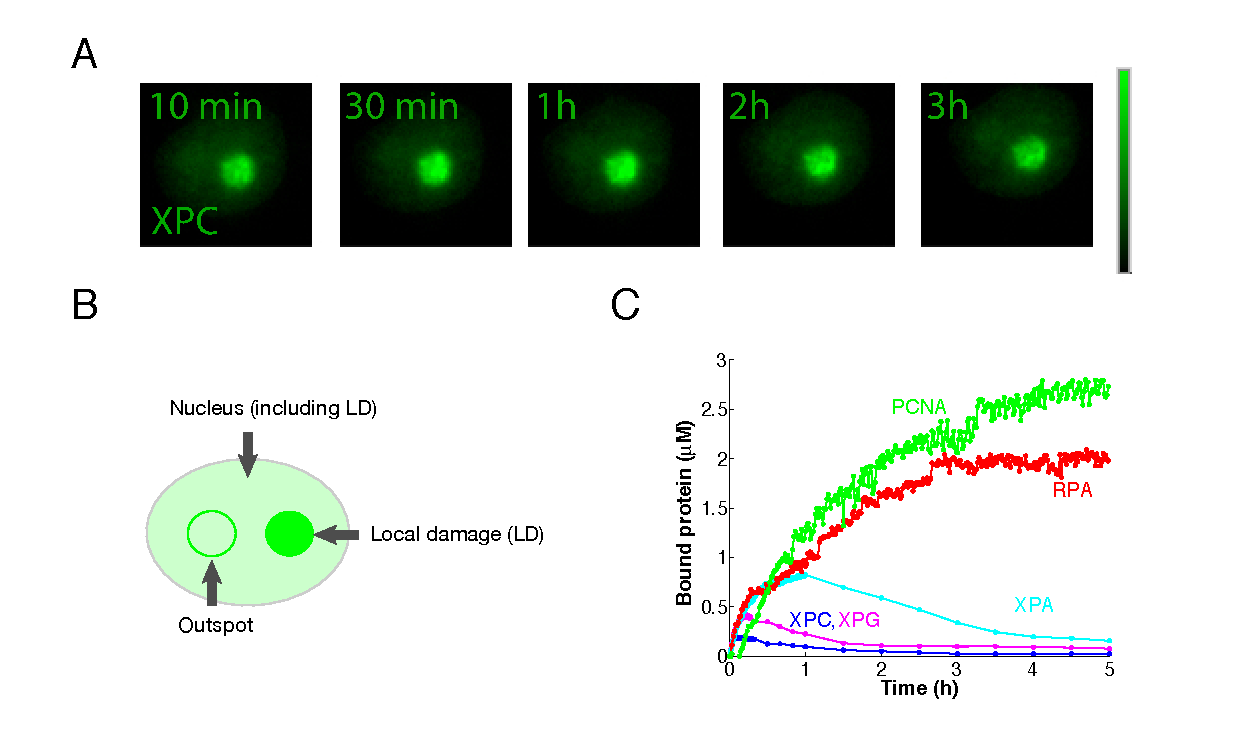
\includegraphics[width=1\textwidth]{Abbildungen/figure2_2.pdf}
\caption{\textbf{Fluorescently labeled NER factors accumulate at locally irradiated nucleus.} A) XPC-eGFP accumulation stably expressed in XP-C cells at different time points after local irradiation with UV-C (100 J$\text{m}^{-\text{2}}$ through 5-\textmu m-diameter pores). B) Scheme of a locally UV-irradiated nucleus. Depicted are all regions relevant for signal quantification. C) Time courses of XPC-eGFP (n = 12), XPG-eGFP (n = 5), eGFP-XPA (n = 7), eGFP-PCNA (n = 5) and RPA-eGFP (n = 5) showing their accumulation at the local damage (LD) spot. For consistency only cell nuclei with one single damage spot were used.}
\label{fig:accuImage}
\end{center}
\end{figure} 
\noindent Each repair factor is tagged with a green fluorescent protein (GFP) (or its 'enhanced' derivative EGFP) and expressed at physiological levels within the cell nucleus. Before the cells are UV-irradiated at time t = 0 the repair proteins are homogeneously distributed. Immediately afterwards the repair factors accumulate at the damaged chromatin sites, which leads to a higher visible fluorescence intensity (cf.\ Figure \ref{fig:accuImage}A). For quantification of the fluorescence intensity image analysis was done by using ImageJ software (NIH Bethesda, MD). Accumulated repair-factor concentrations were determined by multiplying the nuclear reference concentrations (cf.\ Table \ref{tab:nuclearconcentrations}) with the fraction of bound proteins at the damaged DNA:
\begin{equation}
\text{Bound fraction} = (I_\text{LD} - I_\text{outspot})A_\text{LD}/ (I_\text{nucleus} - I_\text{background})A_\text{nucleus}
\label{Eqn:BoundFraction}
\end{equation}     
where $I_\text{LD}$, $I_\text{outspot}$, $I_\text{nucleus}$ and $I_\text{background}$ represent the average fluorescence intensities within the locally damaged spot, an equally sized area in the non-damaged nucleus, the whole nucleus and the background, respectively (cf.\ Figure \ref{fig:accuImage}B). $A_\text{LD}$ and $A_\text{nucleus}$ depict the damaged area and the size of the nucleus. Finally, the concentrations of accumulated protein are calculated assuming a damaged nuclear volume of 0.03 pL.\\   

 \begin{table}[h!]
 \centering
\begin{tabular}{ccc}
\hline
\textbf{Protein} & \quad \textbf{Concentration} \quad& \quad \textbf{Bound fraction}\\ \hline
XPC\hspace{1cm}&0.140 \textmu M&13\%\\ 
TFIIH&0.360 \textmu M&10\%\\  
XPG&0.440 \textmu M&9\%\\  
XPA&1.110 \textmu M&7\%\\  
\quad XPF/ERCC1 \quad&0.170 \textmu M&7\%\\  
RPA&1.110 \textmu M&15\%\\  
PCNA&1.110 \textmu M&20\%\\  \hline
\end{tabular}
 \caption{\textbf{Nuclear concentrations of NER factor in (in \textmu M)} All nuclear quantities are based on published data or on previous estimates \cite{Araujo2001,Houtsmuller1999,Mone2004}. The nuclear concentrations are calculated assuming a nuclear volume of 0.3 pL. The bound
fractionis determined by Eqn. \ref{Eqn:BoundFraction}\cite{Luijsterburg2010}. }\label{tab:nuclearconcentrations}
  \end{table}
  
During the timespan of DNA repair (cf.\ Section \ref{sec:NERexperiments}) NER factors accumulate towards and then gradually decrease from their plateau levels at different rates (cf.\ Figure \ref{fig:accuImage}C). For example the half-life $t_\text{1/2}$ for XPC- and XPG-EGFP is $\sim$1 h whereas $\sim$2.5 h for XPA-EGFP \cite{Luijsterburg2010}. Moreover, PCNA and RPA stay present in the damage spot even after lesion removal. These result show that NER factors engage for hours in the repair process with temporal changes in the molecular composition.\\
To characterize the interaction between repair proteins and DNA intermediates dwell times were determined in fluorescence loss in photobleaching (FLIP) experiments \cite{Luijsterburg2010}. Thereby, a large part of the nucleus, away from the local damage spot, is continuously bleached at 100 \% laser power (cf.\ \ref{fig:accuFlip}A, white rectangle). At the same time fluorescent proteins are probed at low laser power elsewhere within the nucleus. Repair proteins dissociating from the local damage spot have a high probability to be bleached before rebinding due to their large diffusivity. Accordingly, for the dwell time of the repair proteins binding instead of diffusion seems to be rate limiting \cite{Luijsterburg2010}.\\
Still, compared to their long overall presence in the range of hours, all NER factors dissociate very quickly from damaged DNA with half-lives of 20 s (RPA), 25 s (XPC), 50 s (TFIIH, XPG, ERCC1/XPF) and 80 s (RPA) (cf.\ Figure \ref{fig:accuFlip}B). For PCNA the dissociation is strongly biphasic with half-lives of 10 s and 225 s respectively. To analyze, whether the dwell time of slowly accumulating NER factors changes throughout the repair process  resynthesis was stalled by addition of the drugs hydroxyurea (HU) and cytosine-$\beta$-arabinofuranoside. While NER factors reaching their plateau level earlier were not affected \cite{Luijsterburg2010}, omitting the repair progression at this late stage mainly slowed down the dissociation of PCNA and RPA (cf.\ Figure \ref{fig:accuFlip}C). In contrast, XPA's half-life decreased by twofold indicating its higher affinity to repair synthesis intermediates. This shows that the dwell times of NER factors change as repair progresses and suggests that their affinity towards damaged chromatin is defined by the state of the DNA substrate.      
           
  \begin{figure}[htbp]
  	\begin{center}
  		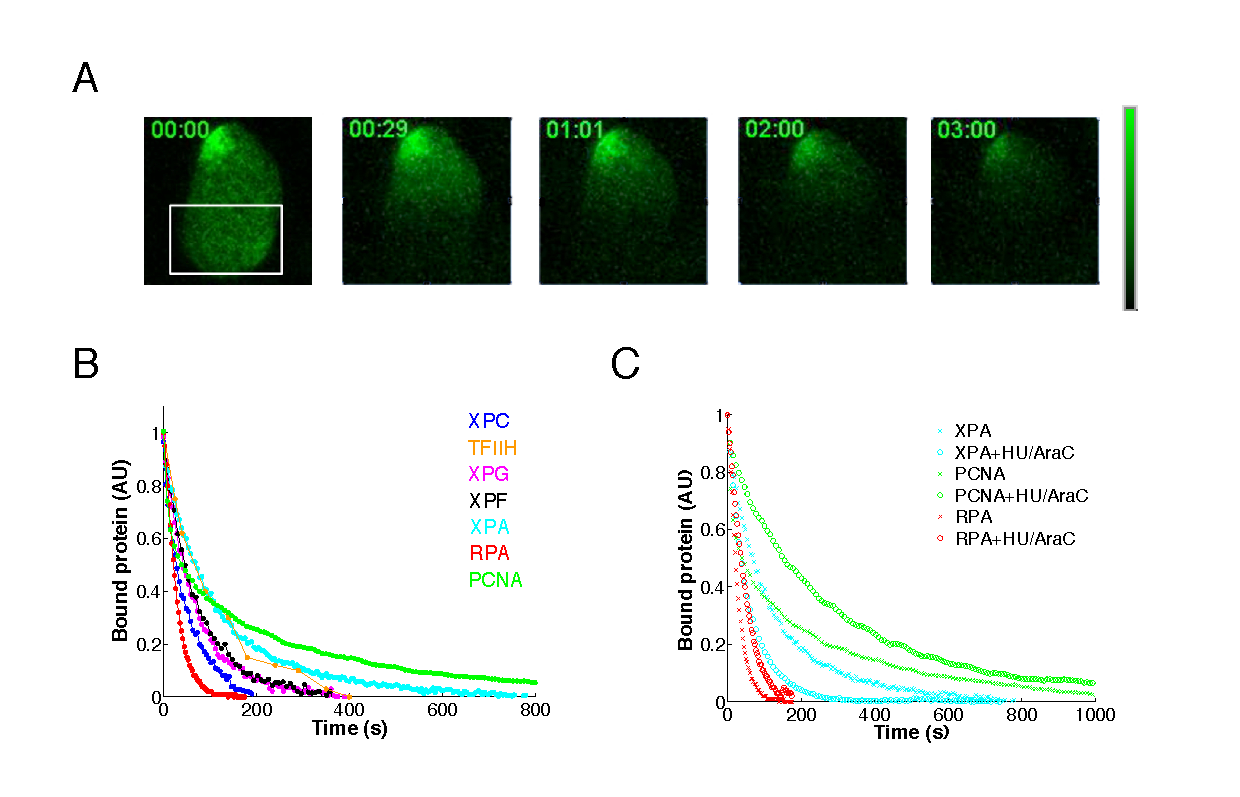
\includegraphics[width=1\textwidth]{Abbildungen/figure2_2_2.pdf}
  		\caption{\textbf{Rapid dissociation of NER factors from damaged DNA.} A) FLIP experiment in XP2OS cells stably expressing eGFP-XPA after 2 h of local irradiation. The nucleus is continuously bleached in an undamaged region (white rectangle). Fluorescence loss is recorded at the sites of local UV-irradiation B) Amount of bound NER-factors (XPC-eGFP, TFIIH-eGFP, XPG-eGFP, XPF-GFP, eGFP-XPA, RPA-eGFP and eGFP-PCNA) monitored over time at LD. C) Quantification of FLIP experiments in the absence or presence of HU and AraC for stably expressed eGFP-XPA, RPA-eGFP and eGFP-PCNA.}
  		\label{fig:accuFlip}
  	\end{center}
  \end{figure}



\subsection{Direct measurement of DNA resynthesis}
\label{Subsec:EdUmeasurement}

In order to expand our quantitative inspection of the NER pathway in intact mammalian cells we established a protocol for the direct measurement of the repair synthesis process. DNA resynthesis reflects the kinetic of the post-incision repair process, complementing the measure of DNA lesion removal, which captures the systems behavior of the pre-incision steps (cf.\ section \ref{sec:NERexperiments}). To visualize newly incorporated DNA shortly before and after local UV irradiation cells were incubated in microscopy medium supplemented with 10 \textmu M 5-ethynyl-2'-deoxyuridine (EdU). Due to its excessive presence in solution the DNA polymerase integrates EdU (a thymidine analog) into the new DNA strand instead of the endogenous thymidine (cf.\ Figure \ref{fig:EdU_measurement}A). After incubation for the desired time cells were fixed stopping EdU incorporation and subsequently permeabilized. EdU is then tagged with the fluorescent azide (AlexaFluor-555, Life Technologies) forming a covalent bond by click chemistry \cite{Limsirichaikul2009}. Analogous to the quantification of NER factor dynamics EdU intensities were captured with a laser scanning microscope (Zeiss).\\
Accordingly, incorporated EdU is exclusively present at the locally confined area of  damaged DNA, which coincides with the localization of immunostained XPC (cf.\ Figure \ref{fig:EdU_measurement}B, upper row). The same result occurs for XP-C cells with stably transfected XPC-eGFP (cf.\ Figure \ref{fig:EdU_measurement}B, lower row). Replicating cells could be excluded easily from the analysis due to there prevalent EdU incorporation distributed over the entire nucleus. 
  

    
 


\begin{figure}[htbp]
\begin{center}
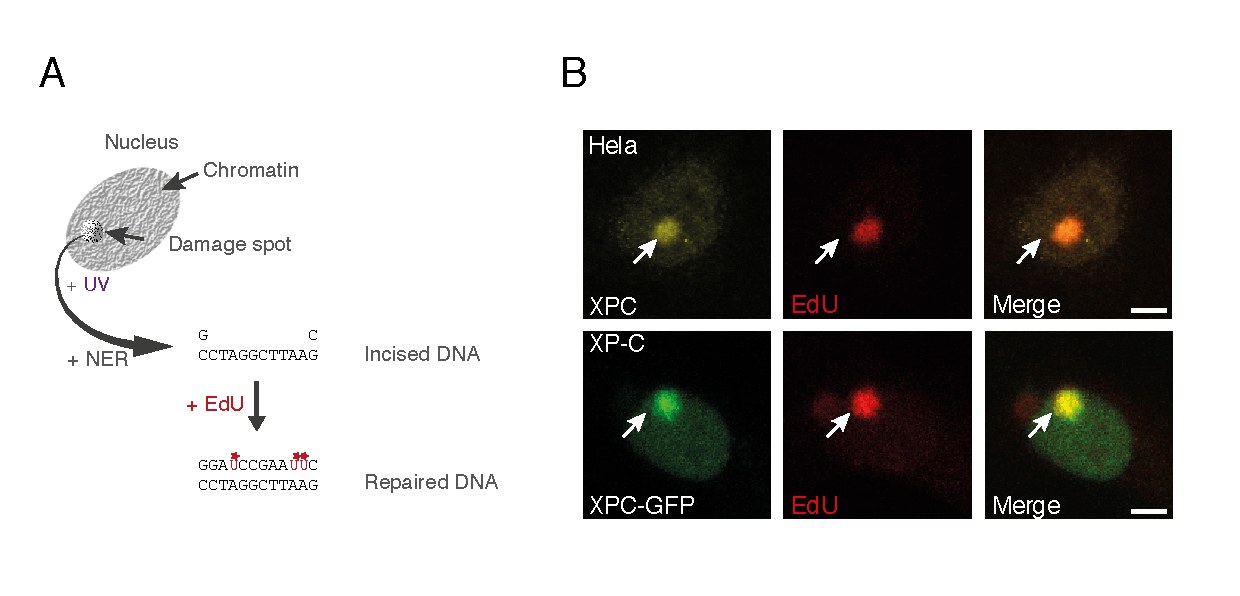
\includegraphics[width=1\textwidth]{Abbildungen/figure2_3.pdf}
\caption{\textbf{EdU is incorporated at sites of local DNA damage.} A) Schematic illustration depicting the experimental procedure of EdU incorporation of locally damaged cells. B) Endogenous XPC in Hela cells (upper panel) or stably express XPC-eGFP (lower panel) accumulate in the LD spot and co-localize with incorporated EdU.}
\label{fig:EdU_measurement}
\end{center}
\end{figure}


\subsection{Repair rate follows first order rate kinetic}
\label{firstOrderRateKinetic}
In contrast to the real time measurements for accumulation and dissociation of the NER factors the incorporation of EdU cannot be followed continuously. As mentioned in section \ref{Subsec:EdUmeasurement} cells have to be fixed and permeabilized before the newly incorporated bases can be fluorescently labeled. Therefore, only the accumulated EdU incorporated in the time interval between UV-irradiation and fixation can be followed. By repeating this procedure for growing time intervals we acquired successively the repair kinetic for newly repaired DNA (cf.\ Figure \ref{fig:DNArepairKinetic}A and B). For each time point we averaged over multiple cells. \\
We found that EdU incorporation essentially stops after 4 h, which coincides with the removal of 6-4PP (cf.\ \cite{Luijsterburg2010} and Figure \ref{fig:DNArepairKinetic}B red and blue curve, respectively). This agrees with the observation that NER is not primarily engaged in the removal of cyclobutane pyrimidine dimers (CPD) which are repaired on a much longer timescale. To test whether the availability of EdU is rate limiting we measured the incorporation of EdU in discrete equidistant time intervals after UV-irradiation (cf.\ Figure \ref{fig:DNArepairKinetic}C and Appendix XX). As it turns out the amount per time interval of EdU incorporation is indeed continuously declining and hence the rate of repair synthesis. Moreover the EdU kinetic follows the trajectory of PCNA accumulation as measured by Luijsterburg \textit{et al.} \cite{Luijsterburg2010} (cf.\ Figure \ref{fig:DNArepairKinetic}D). PCNA in turn is thought to act as processivity factor for the DNA polymerase and remains bound to the DNA \cite{Luijsterburg2010,Essers2005,Sporbert2002}. Taken together, these data establish EdU incorporation as a direct and quantitative measure of DNA repair synthesis in locally damaged cells.\\
The DNA repair time series characterized by incorporated EdU is fitted by a mono-exponential kinetic (cf.\ Figure \ref{fig:DNArepairKinetic}E):
\begin{equation}
EdU(t) = EdU_\text{max}(1 - e^{\lambda t}),
\label{Eqn:EdU_kinetic}
\end{equation}  
where $EdU(t)$ and $EdU_{\text{max}}$ depict the amount of incorporated EdU and its value at saturation, respectively. The time constant is $\lambda$=0.58 ($\pm$0.07) $\text{h}^{-\text{1}}$. This result indicates that, despite its molecular complexity, 6-4PP removal by NER is a slow first-order reaction with a half-time of 1.2 hours.          
\begin{figure}[b!]
\begin{center}
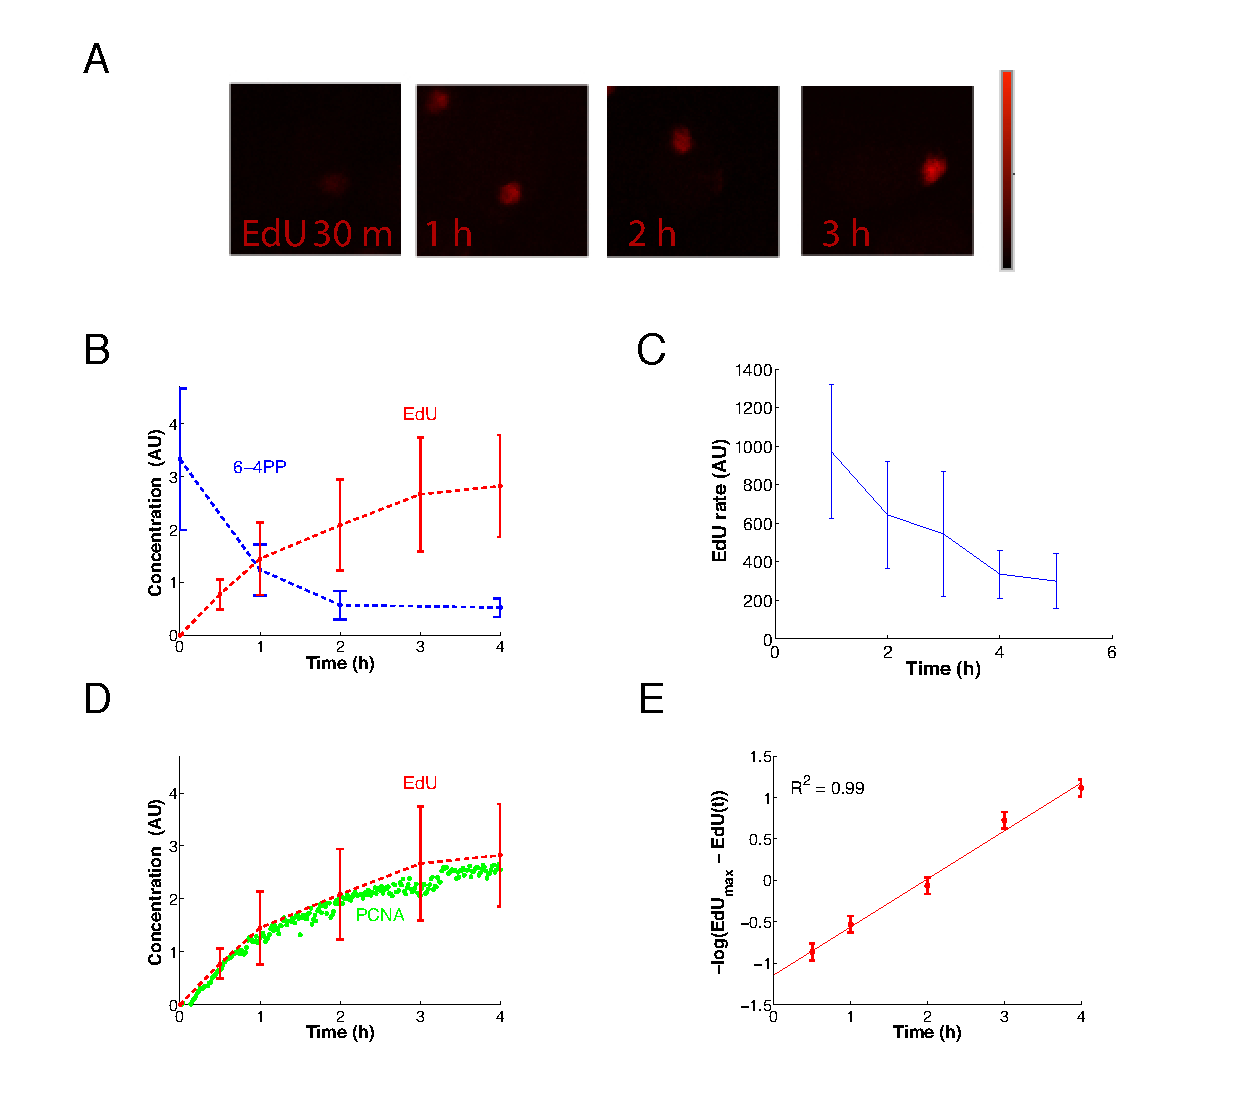
\includegraphics[width=1\textwidth]{Abbildungen/figure2_4.pdf}
\caption{\textbf{EdU incorporation reflects DNA repair synthesis quantitatively.} A) EdU signal at various time points after local UC-C irradiation. B) Repair DNA synthesis (EdU, red curve) coincides with damage removal (6-4PP, blue curve) measured previously by Luijsterburg \textit{et al.} \cite{Luijsterburg2010}. The EdU trajectory represents mean $\pm$ SD (derived from three independent experiments) of DNA repair in n=150 locally damaged cells per time point. C) D) DNA repair synthesis follows PCNA accumulation as measured previously \cite{Luijsterburg2010}. E) Mono-exponential fit of the EdU kinetic according to Eqn. \ref{Eqn:EdU_kinetic}.}
\label{fig:DNArepairKinetic}
\end{center}
\end{figure}

\section{Kinetic model of NER}
\subsection{Slow first-order reaction kinetic due to many fast interacting components}
\label{sec:toyModel}
To investigate the mechanistic connection between fast NER factor exchange at the DNA template and the overall slow repair time it appears practical to apply an analytical approach. During her Ph.D. thesis Gesa Terstiege together with Thomas H\"ofer performed this analysis \cite{Terstiege2010,Verbruggen2014}, considering the complex formation with a simplified model including $N$ repair factors. They examined different scenarios distinguishing random and sequential protein assembly; reversible and irreversible protein binding or mixed mechanisms specific for each DNA repair intermediate. Under appropriate assumptions, the mean repair time of such a process can be generally expressed with:

\begin{equation}
\tau = \underbrace{\frac{1}{k}\sum^{N-1}_{i=0}A_i\left(\frac{l}{k}\right)^i}_{\text{first assembly}} +  \underbrace{\frac{1}{\rho}\sum_{i=0}^{N}B_i \left(\frac{l}{k}\right)^i}_{\text{reassembly and reaction}} \label{Eqn:taugen}
\end{equation}

where $k$ denotes the pseudo-first order association rate constant of NER factors, $l$ the dissociation rate constant of NER factors and $\rho$ the rate of the repair reaction (cf.\ Figure \textbf{tbd}A,\cite{Verbruggen2014}). $A_i$ and $B_i$ differ between random assembly
\begin{equation}
A_i^\text{rand}= \sum_{j=1}^{N-i}\frac{1}{i+j}\frac{{N \choose j-1}}{{N\choose i+j}} , \quad B_i^\text{rand} = {N\choose i},\label{Eqn:coefrand}
\end{equation} 
and sequential assembly           
\begin{equation}
A_i^\text{seq}= N-i , \quad B_i^\text{seq} = 1.\label{Eqn.coefseq}
\end{equation}
Sequential and random assembly occur on a similar time scale for a number of repair components smaller than 10 considering reversible protein binding ($l=k=1$) \cite{Terstiege2010}, which coincides with the number of core NER factors \cite{Luijsterburg2010}. The theoretical component number for equal repair times is even higher for increasing reaction rates ($\rho \gg k,l$). Given that all repair factor dwell times are in the order of $\sim$1 min ($k$ = $l$ = 1 $\text{min}^{-\text{1}}$) the model was simulated for N = 9 components (cf.\ Figure \textbf{tbm}C). Remarkably, the resulting trajectory followed a single-exponential kinetic with a half time of $\sim$1 hour in case of balanced reversibility. In contrast, for an irreversible process ($l/k = 0$) the repair kinetic resembles a sigmoid time course (cf.\ Figure\textbf{tbm}B). These results suggest that the rapidly exchanging NER factors naturally generate a mono-exponential repair kinetic whereas the slow overall time span can be explained by the stochastic distribution of repair events.

\begin{figure}[h]
\begin{center}
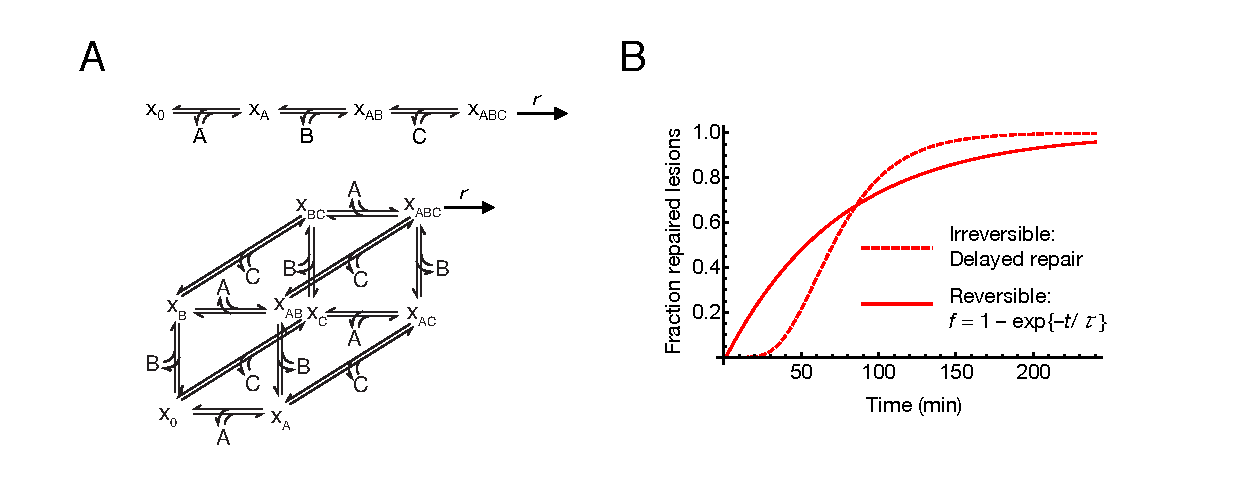
\includegraphics[width=1\textwidth]{Abbildungen/figure2_5_2.pdf}
\caption{\textbf{Simplified analytical model of the repair complex formation} A) Sequential (above) and random (below) assembly scheme of the repair factors A, B and C to the DNA template $\text{x}_i$. $\text{x}_0$ denotes the empty lesion (e.g. damaged DNA). When the complex is fully assembled ($\text{x}_{\text{ABC}}$) it performs a catalytic repair step with rate $r$. B) Simulated repair time courses for random reversible (solid line) and irreversible (dashed line) repair factor assembly. For reversible binding ($k=l= \text{1 min}^{-1}, N=\text{9}$) the trajectory fits a mono-exponential repair kinetic with time constant $\tau$ whereas for irreversible binding the fit has sigmoidal shape ($l=\text{0}, k=\text{0.037 min}^{-1}, N=\text{9}$, chosen to get the same time constant).}
\label{fig:reactionTiming}
\end{center}
\end{figure}


\subsection{Model structure and parametrization}
To examine the relation between rapid repair factor exchange and the slow first-order reaction kinetic we extended this analysis on the basis of a realistic NER model. Conceptually, it follows a model worked out by Luijsterburg \textit{et al.} (2010) \cite{Luijsterburg2010}. According to this, NER factors bind transiently to DNA repair intermediates thereby forming catalytic complexes that, if complete, perform the next repair step. These are usually irreversible reactions embodying the sequential characteristics of this pathway (cf.\ Figure \textbf{tbm}).\\
The nature of these distinguishable repair intermediates is widely investigated in biochemical but also in \textit{in vivo} studies \cite{Evans1997a,Mu1996,Polo2006,Tapias2004}.
Accordingly, the evolved model distinguishes five DNA repair intermediates: i) damaged DNA, unwound DNA, incised DNA, resynthesized DNA and rechromatinized DNA. The molecular state of these intermediates defines the binding affinity for a specific set of repair proteins (cf.\ Figure \ref{fig:ModelStructure}). Table \ref{tab:modelassumptions} summarizes all repair intermediates and lists the corresponding repair factors that show affinity for a particular repair intermediate. Repair factors that catalyze the enzymatic reaction if assembled are indicated. As stated before, FLIP measurements indicate that diffusion is not rate limiting for protein binding and thus not included in the model (cf.\ Section \ref{subsec:AccuFlipExp} and \cite{Rademakers2003,Zotter2006}).              


\begin{figure}[t!]
\begin{center}
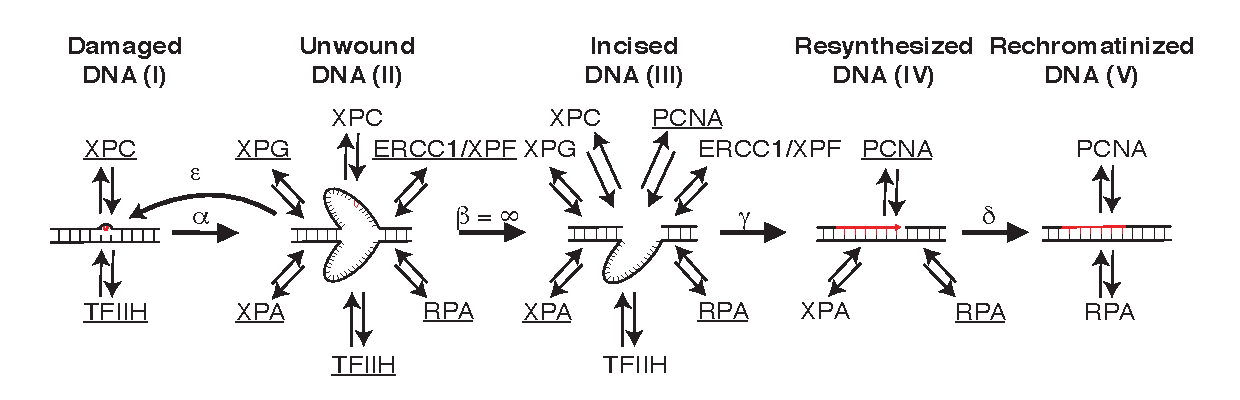
\includegraphics[width=1\textwidth]{Abbildungen/figure2_5.pdf}
\caption{\textbf{Schematic model description of the DNA repair mechanism.} The model distinguishes five individual repair intermediates: Damaged (I), unwound (II), incised (III), resynthesized (IV) and rechromatinized DNA (V). As indicated, specific tuples of repair proteins bind reversibly to the intermediates. Catalytic reactions, denoted by Greek letters, occur when the particular reaction complex (underlined proteins) is assembled. }
\label{fig:ModelStructure}
\end{center}
\end{figure}
A prominent role within the NER pathway belongs to the lesion recognition factor XPC. Theoretical results suggest that the detection of damaged DNA sites by a single element instead of multiple simultaneously is crucial for the efficient initiation of the repair process \cite{Politi2005}. Beside this exception the model allows random, non-cooperative binding binding for all NER factors subsequently assembling at the chromatin.\\    
The model structure introduced above and shown in Figure \ref{fig:ModelStructure} was translated into an ordinary differential equation system assuming mass-action kinetics for all protein-DNA interaction processes. Each equation describes the concentration of a single DNA state $y_{\pi}^{R}$ (cf.\ Eqn. \ref{eqn:DNAstatesModel}) associated with a specific repair intermediate R = I, II,...,V (damaged (I), unwound (II), incised (III), resynthesized (IV), rechromatinized (V)). The index $\pi$ represents a binary vector where each position displays the presence or absence of a repair protein p (p $\in$ {C, T, G, A, F, R, P}, where XPC (C), TFIIH (T), XPG (G), XPA (A), ERCC1/XPF (F), RPA (R) and PCNA (P)). $\pi(p)=1$ if protein p is bound and $\pi(p)=0$ if not. The length of $\pi(p)$ is defined according to the model structure (cf.\ Table \ref{tab:modelassumptions}) with: $\pi_{R=I} = \{ \text{C,T} \}$; $\pi_{R=II} = \{ \text{C,T,G,A,F,R} \}$; $\pi_{R=III} = \{ \text{C,T,G,A,F,R,P} \}$; $\pi_{R=IV} = \{ \text{A,R,P} \}$; $\pi_{R=V} = \{ \text{R,P} \}$. The time course of this model is then described by:

\begin{equation}\label{eqn:DNAstatesModel}
\frac{d}{dt}\;y_{\pi}^{R} =\sum_{p\text{ in }R}\eta \, \left( (-1)^{\pi(p)} \,l_{p}^{ R}\, y_{\pi}^{R}\left. \right|_{\pi(p)=1}+  \, (-1)^{1+\pi(p)}\, k_{p}^{ R} \,C_p(t)\,y_{\pi}^{R}\left. \right|_{\pi(p)=0}\right ) +E(y_{\pi}^{R}),
\end{equation}\\
where $\eta$ represents a cooperativity ensuring the exclusion of all cooperative binding events:
\begin{align*}
\eta =\left\{
\begin{array}{llll}
& =\; 0 \quad   &\text{if}& R=\text{I} \wedge p=\text{C} \wedge \text{T}=1, \\
&     && R=\text{I} \wedge p=\text{T} \wedge \text{C}=0,\\
& = \; 1 \quad &\text{else}.&
\end{array}
\right.
\end{align*}
  
The kinetics describing protein exchange at the repair intermediates are characterized by the binding constant $k_{p}^{ R}$ and the dissociation constant $l_{p}^{ R}$. The free protein concentrations are denoted by $C_p(t)$ representing seven additional differential equations for $p \in \{\text{C,T,G,A,F,R,P}\}$:

\begin{eqnarray}\label{Eqn:concentration}
\frac{d}{dt}\;C_p&=&\,\sum_{R=\text{I}}^{\text{V}} \sum_{\pi} \xi \left( \,\delta_{\pi (p)1}\;l_{p}^{ R}\, y_{\pi}^{R}- \,\delta_{\pi (p)0}\; k_{p}^{ R} \,C_p\,y_{\pi}^{R}\right)
\end{eqnarray}  

Analogous to $\eta$, $\xi$ governs the sequential binding of XPC and TFIIH by:

\begin{align*}
\xi =\left\{
\begin{array}{l l ll}
& =\; 0 \quad   &\text{if} & R=\text{I} \wedge \text{C}=0 \wedge \text{T}=1, \\
&    && R=\text{I} \wedge p=\text{C} \wedge \text{C}=\text{T}=1, \\
&    &&R=\text{I} \wedge p=\text{T} \wedge \text{C}=\text{T}=0, \\
& = \; 1 \quad& \text{else }.&
\end{array}
\right.
\end{align*}

\begin{table}[h]
	\small{
		\begin{tabular}{cccccc}
			\hline
			\rule{0pt}{2ex}
			\textbf{Repair}&\textbf{Binding} &	\textbf{Catalyzed  process}&\textbf{Remarks}  	&\textbf{Ref.} \\ 
			\textbf{intermediate}&	\textbf{proteins} &	\textbf{Required proteins}&	& \\ \hline
			\rule{0pt}{3ex}
			(I) Damaged DNA&	XPC,TFIIH 	&Unwinding &Initiation by binding	&\cite{Evans1997a}
			\\ 
			 &	(3 states)& (reaction $\alpha$)&  of XPC and subsequent &\cite{Riedl2003}\\
			&&XPC and TFIIH&	 recruitment of TFIIH. &\cite{Yokoi:2000:J-Biol-Chem:10734143}\\ 
			&&&&\cite{Rademakers2003}\\ 
			&&&& \cite{Volker2001} \\ 
			&&&&\\\hline
			\rule{0pt}{3ex}
			(II) Unwound DNA&XPC,TFIIH,&Dual incision &If the DNA becomes &\cite{Evans1997a} \\
			& XPG, XPA,&(reaction $\beta$)&devoid of any protein,&\cite{ODonovan:1994:Nature:8090225}\\
			&ERCC1/XPF,&TFIIH,XPG,&it will re-anneal (reaction &\cite{Sijbers:1996:Cell:8797827}\\
			&  RPA& XPA,  RPA&$\varepsilon$). Dual incision requires&\cite{Winkler2001}\\
			&(64 states)&and ERCC1/XPF&the endonucleases XPG& \cite{deLaat:1998:Genes-Dev:9716411}\\
			&&&  and ERCC1/XPF and is&\\
			&&&stimulated by TFIIH, &\\
			&&&XPA, RPA and possibly &\\
			&&&XPC.&\\
			&&&& \\ \hline
			\rule{0pt}{3ex}
			(III) Incised&XPC,TFIIH,&Repair-synthesis&PCNA binds to the free&\cite{Evans1997a}\\
			DNA& XPG, XPA,& (reaction $\gamma$)&3'-OH group generated by&\cite{Winkler2001}\\
			& ERCC1/XPF,&XPA, RPA and&  the ERCC1/XPF incision.&\\
			&RPA, PCNA& PCNA& DNA polymerase is also&\\
			&(128 states)&& required (not measured).	&\\
			&&&& \\   \hline
			\rule{0pt}{3ex}
			(IV) Resynthesized&XPA, RPA,&Rechroma-&Accumulation&\cite{Moser2005}\\
			DNA&	 PCNA& tinization& data imply that XPA&  \cite{Shivji:1995:Biochemistry:7711023}\\
			&(8 states)&(reaction $\delta$)& binds  to repaired DNA &\cite{Luijsterburg2010}\\
			&&RPA and PCNA&while the pre-incision &\\
			&&&	  proteins do not &\\
			&&& (Figure \ref{fig:accuImage}C).&\\
			&&&& \\ \hline
			\rule{0pt}{3ex}
			(V) Rechromatin- &RPA, PCNA &&RPA and PCNA associate&\cite{Riedl2003}\\
			ized DNA &(4 states)	&&with rep. intermediate $I$,&\cite{Luijsterburg2010}\\
			&&&as levels of bound EGFP-&\\
			&&&PCNA and EGFP-RPA&\\ 
			&&& are  high up to at least 4h&\\
			&&& after UV irradiation while&\\
			&&& other repair proteins are&\\   
			&&& no longer bound.&\\   &&&& \\ \hline
		\end{tabular}}
		\caption{\textbf{Model assumptions.} Adapted from Terstiege \textit{et al.} (2010) \cite{Terstiege2010}}\label{tab:modelassumptions}
	\end{table}\clearpage
	


Finally, if an enzymatic complex has fully assembled at the DNA template it catalyzes the next repair step, which is represented in the model with the term $E(y_{\pi}^{R})$. After damage recognition by XPC damaged DNA is unwound by the helicase TFIIH with the unwinding activity $\alpha$, whereas XPC acts as a stabilizing/proof reading factor in parallel.  
%clarify what role plays XPC in this context...
Accordingly $E(y_{\pi}^{R})$ translates into the following catalytic reactions for damaged DNA ($R= \text{I}$):
$$E(y_{00}^\text{I})=\;\varepsilon\;y_{000000}^\text{II} \quad \text{ and }\quad
E(y_{11}^\text{I})=\;-\alpha \;y_{11}^\text{I},$$
If all proteins fall off the DNA template due to false damage detection the DNA will re-anneal with the rate $\epsilon$. Otherwise a complex formed by TFIIH, XPG, XPA, XPF, XPA and RPA will eventually promote the excision of the lesion DNA strand leading to the following catalytic reactions for unwound DNA ($R= \text{II}$): 

\begin{align*}
	\begin{array}{l l llll}
		E(y_{000000}^\text{II})&=&-\;	\varepsilon	\;y_{000000}^\text{II}\;, &E(y_{110000}^\text{II})&=\;	\alpha	\;y_{11}^\text{I},\\
		\text{ and }&&    & E(y_{011111}^\text{II})&=-\	\beta	\;y_{011111}^\text{II}.
	\end{array}
\end{align*}

Once the lesion strand is excised with incision rate $\beta$ the remaining repair steps are irreversible. Incised DNA is resynthesized with the rate $\gamma$ by the resynthesis complex  XPA-RPA-PCNA. XPA is assumed to assemble at post incision repair intermediates as suggested by experiments with inhibited incision that showed accelerated dissociation FLIP kinetics for XPA  \cite{Luijsterburg2010}. This result is supported by a chromatin immunoprecipitation (ChIP) experiment with antibodies against XRCC1- Lig III showing the co-precipitation of XPA and RPA but not XPC and TFIIH \cite{Moser:2007:Mol-Cell:17643379}. Evidence for the importance of PCNA and RPA for the resynthesis reaction was shown by Shivji \textit{et al.} (1995) \cite{Shivji:1995:Biochemistry:7711023}. This results into the following catalytic reactions for incised DNA ($R= \text{III}$):  
            
\begin{align*}
\begin{array}{l l llll}
E(y_{1111111}^\text{III})&=&\;	\beta \;	y_{011111}^\text{II}	 \quad \text{and}
&E(y_{0001011}^\text{III})=&\;	-\gamma	\;y_{0001011}^\text{III}.	 \\
\end{array}
\end{align*}

In correspondence to the previously described accumulation measurements (cf.\ Figure \ref{fig:accuImage}) only RPA and PCNA stay bound during chromatin remodeling, the last modeled repair intermediate. This leads to the following enzymatic reactions for resynthesized DNA  ($R= \text{IV}$) and rechromatinize ($R= \text{IV}$):


\begin{align*}
\begin{array}{l l llll}
E(y_{111}^\text{IV})&=&\;	\gamma \;	y_{0001011}^\text{III},	 
&E(y_{011}^\text{IV})=&\;	-\delta	\;y_{011}^\text{IV},	 \\
\text{and} && & E(y_{11}^\text{V})= &\;	\delta	\;y_{011}^\text{IV}.
\end{array}
\end{align*}

Since all NER factors can bind independently the DNA template for each repair intermediate there are a total of $ 2^N $ repair states where $ N $ is the number of repair proteins assembling to the particular repair intermediate. Due to the sequential assembly of TFIIH after lesion detection of XPC the number of states for damaged DNA is reduced to $ 2^2-1 = 3$ states. For the remaining repair intermediates we derive  $ 2^6 = 64$ for unwound DNA; $ 2^7 = 128$ states for incised DNA; $ 2^3 = 8$ states for resynthesized DNA and $ 2^21 = 4$ states for rechromatinized DNA. This results in a total of 214 states including seven differential equations for the free NER-factor protein concentrations. \\
Summing over all repair states and the respective intermediates associated to one repair factor we can simulate the its accumulation kinetic. As initial conditions serve the measured free protein concentrations denoted in Table \ref{tab:nuclearconcentrations}\cite{Terstiege2010,Luijsterburg2010} and the initial amount of inflicted damages whose concentration was estimated with  $y_{00}^{\text{I}} = 3.33$ \textmu M. The remaining states start at zero. To reproduce the FLIP kinetic for a specific repair factor all corresponding dissociation constants were set to zero at the time of maximal accumulation when the FLIP experiment started. Accordingly FLIP kinetics were acquired after 600 s for XPC and ERCCC1/XPF, 900 s for XPG and TFIIH and 2000 s for XPA and 7200 s for PCNA. 

 
\section{Maximum likelihood approach together with PLE analysis identifies realistic model of NER}
\subsection{A maximum likelihood approach for efficient model fitting}
\label{sec:maximumLL}
To find a realistic parameterization for the temporal development of the repair states $y_\pi^R$ (cf.\ Eqn. \ref{eqn:DNAstatesModel}) the model was mapped to $m$ observables via a function $f_z$:

  \begin{equation}
  	z(t_i,\theta) = f_z(t_i,y(t_i,\theta),\theta).
  	\label{eqn:observable}
  \end{equation} 

The observables $z$ are parameterized by $\theta$ and resemble experimentally derived quantities at time $t_i$. $\theta$ depicts binding, dissociation and catalytic constants adding up to a total of 45 model parameters. Each observable $z_k(t_i,\theta)$ corresponds to the measured data $z_k^\dag(t_i)$ with intrinsic noise $\epsilon_{ki}$. Its origin can be traced back to a mixture of measurement noise combined with the naturally occurring biological variability. Assuming additive, normally distributed noise leads to $z_k(t_i)^\dag = z_k(t_i,\theta) + \epsilon_{ki}$ with $\epsilon_{ki} \sim N(0,\sigma_{ki}^2)$. To calibrate the measured data $z_k(t_i)^\dag$ with the model observables $z_k(t_i,\theta)+\epsilon_{ki}$ we applied a maximum likelihood approach as distance measure which translates for normally distributed noise into:
\begin{equation}
\label{eqn:likelihood}
L(z^\dag \textbar \theta) = \varPi_{k=1}^m \varPi_{i=1}^{d_k} \frac{1}{\sqrt{2\pi \sigma_{ki}^2}}\exp \left( -\frac{1}{2\sigma_{ki}^2}\left(z_{ki}^\dag - z_k(t_i,\theta)\right)^2\right)
\end{equation}
  
Here, $d_k$ denotes the number of distinct experimental data sets $z^\dag$ for each observable $k\sim 1 ...m$, measured at time points $t_i$ with $i\sim 1 ... d_k$. $\sigma_{ki}^2$ are the variance components of the measurement noise of each data point. Instead of maximizing the likelihood it is equivalent and numerically more efficient to minimize its negative logarithm $-2log(L(z^\dag\textbar\theta))$ instead. In the following we will refer to it as $X^2$.  For the minimization of the $X^2$ the choice for $\theta$ is controlled by $\sigma_{ki}^2$ (cf.\ Eqn. \ref{eqn:likelihood}). As shown by Raue and colleagues for the reliable estimation of the model parameters $\theta$ the simultaneous approximation of $\sigma_{ki}^2$ together with the model dynamics leads to a statistically more accurate assessment of the model parameters than using noise estimations from preprocessed data \cite{Raue2013}. Accordingly $\sigma_{ki}^2$ can be considered as parameterized function

\begin{equation}
\sigma_{k}(t_i,\theta) = f_{\sigma_{k}}(t_i,z(t_i,\theta),\theta).
\end{equation}    

wherein additional parameters are introduced representing the type and magnitude of the modeled noise. Analogous we applied an additive error model for each observable with the parameterized function $\sigma_{k}(t_i,\theta) = s_a$ and $\epsilon_{ki} \sim N(0,\sigma_{ki}^2)$ where $s_a$ is included in $\theta$.\\ 
For reasons of fitting-speed efficiency we implemented our model into the online-available D2D software environment \cite{Raue2013} optimized for MATLAB (2011a, The Mathworks Inc., Natick, MA). The integrated fitting procedure applies the trust region algorithm LSQNONLIN, which is pre-implemented in MATLAB. The algorithm requires the derivatives of the objective function with respect to the parameters (cf.\ Eqn. \ref{eqn:likelihood}). The inner derivatives $dy(t,/theta)/d\theta$, also called sensitivities, provide gradient information about the parameter landscape and thus are crucial to guide the optimization algorithm to the nearest optimum. The sensitivities can be passed in form of sensitivity equations 

\begin{equation}
	\frac{d}{dt}\frac{dy(t,\theta)}{d\theta} = \frac{\partial f_y}{\partial y}\frac{dy(t,\theta)}{d\theta}+\frac{\partial f_y}{\partial \theta},
\end{equation}  

which represent additional ODEs that are solved in parallel to the original ODE system (cf.\ Eqn. \ref{eqn:DNAstatesModel})\cite{Leis1988}. Applying sensitivity equations instead of a simple finite difference approximation proved to be numerically more accurate and computationally also faster \cite{Raue2013}. Both, model and sensitivity ODEs were solved with the CVODES algorithm written in ANSI (\textbf{don't forget in the abbreviations list}) standard C \cite{Hindmarsh2005}. \\
To avoid terminating the optimization procedure in a local minimum we used a 'multi-start' approach by drawing the initial parameter vector systematically using Latin hypercube sampling (LHS) \cite{Owen2014}. In contrast to a random sampling approach LHS provides a better coverage of the sampling space by maximizing the distance between successive parameter draws \cite{Raue2013}.    

\begin{figure}[htbp]
\begin{center}
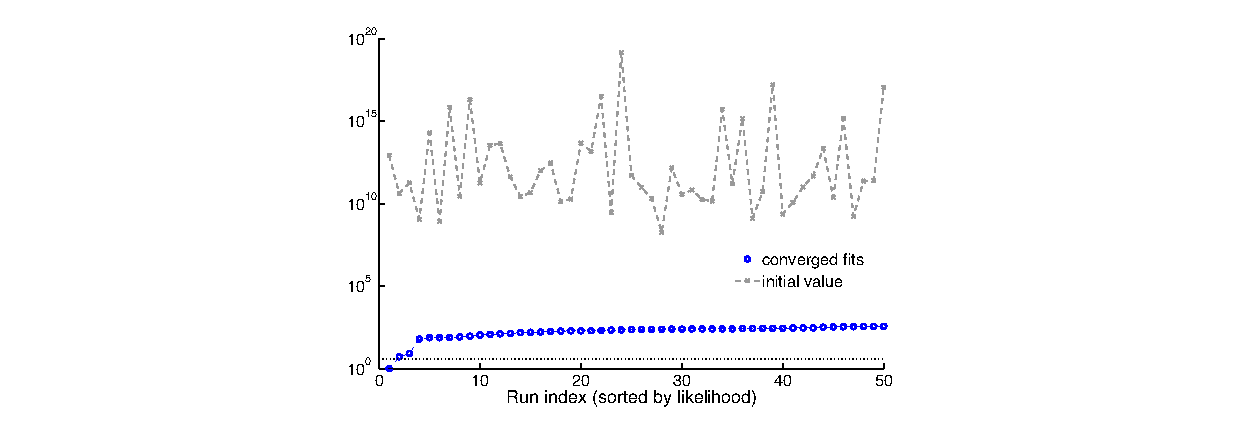
\includegraphics[width=1\textwidth]{Abbildungen/figure2_6_4.pdf}
\caption{\textbf{Parameter estimation for the 50 best fits after initial Latin hypercube sampling} Visualization of performance using 50 independent optimization runs (blue dots depict final optima of each individual run). Initial guesses (grey stars) were generated by Latin hypercube sampling. For illustrative purposes the global optimum is centred to 1. \textbf{put objective function on the left/axis handles bigger...} }
\label{fig:LHS}
\end{center}
\end{figure} 

\begin{figure}[htbp]
\begin{center}
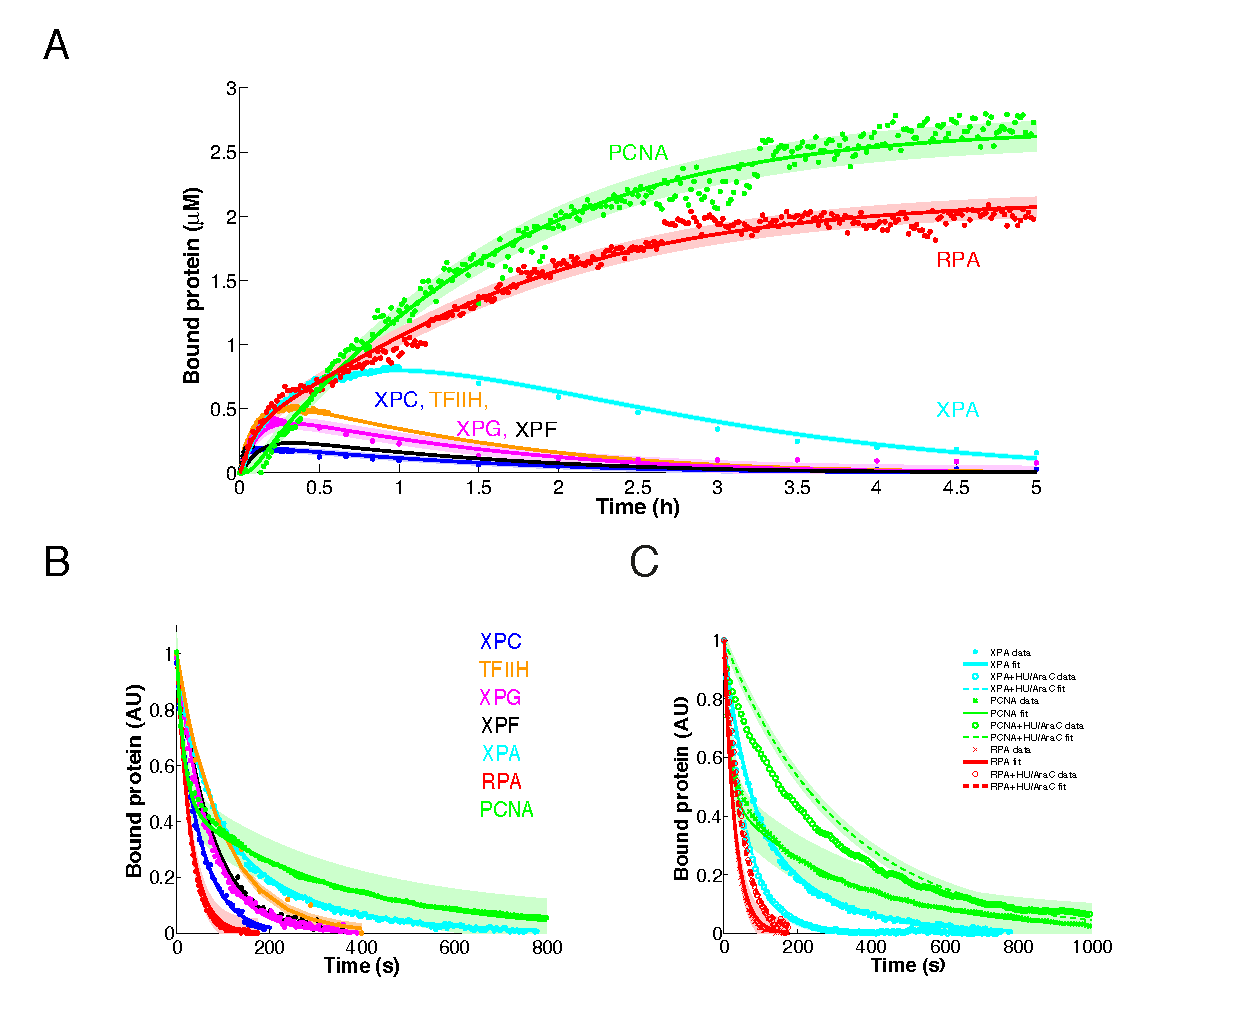
\includegraphics[width=1\textwidth]{Abbildungen/figure2_6.pdf}
\caption{\textbf{Quantitative NER model fits to accumulation and dissociation time courses.} A and B) Simulation (lines) and measurement (dots) of the accumulation and dissociation kinetics for the repair factors XPC, TFIIH, XPG, XPA, XPF, RPA and PCNA. Estimated errors are depicted as shaded area. C) Fitted FLIP time courses of XPA, RPA and PCNA in the absence or presence of AraC and HU on locally irradiated cells.)}
\label{fig:ModelFit_accu_flip}
\end{center}
\end{figure}

\subsection{NER model fits accumulation, FLIP and repair synthesis measurements}    

To derive faithful fitting results we reiterated the optimization process for 250 times. For each iteration the starting parameters were redrawn by Latin hypercube sampling. Despite the size of the model, with respect to data points and the number of parameters, the majority of fits terminated relatively close to the global $X^2$ minimum (cf.\ Figure \ref{fig:LHS}) give percentage of the difference). Nevertheless two distinct minimums can be distinguished suggesting a close local minimum, which 'hides' the rarely reached global minimum. For both parameter sets the model fits the experimental data set comprising accumulation, FLIP, perturbation and repair synthesis measurements with small estimated measurement errors (cf.\ Figure \ref{fig:ModelFit_accu_flip}A, B, C). The accumulation kinetics (cf.\ Figure \ref{fig:ModelFit_accu_flip}A) are depicted as concentrations scaled by the volume of the locally damaged area which was assumed to be 10\% of the nuclear volume. We believe that this specification is more intuitively comprehensible  compared to scaling by the whole nuclear volume as performed by Luijsterburg \textit{et al.}\cite{Luijsterburg2010}. Moreover it allows the realistic comparison between simulated and measured microscopy images of NER factor accumulation and EdU incorporation (cf.\ Figure \ref{fig:Fitt_accu_Mic}).  

\begin{figure}[htbp]
\begin{center}
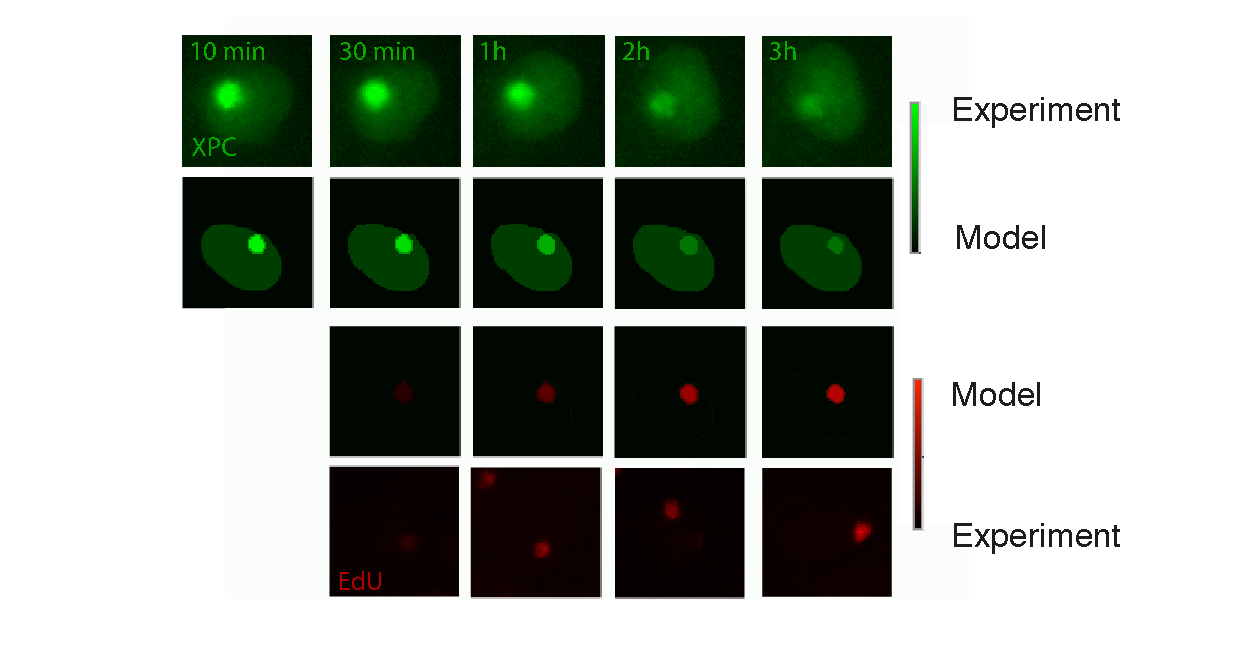
\includegraphics[width=1\textwidth]{Abbildungen/figure2_6_2.pdf}
\caption{\textbf{Comparison between measured and simulated single cell microscopy images} Simulated time courses (lines) and the associated microscopy images for GFP tagged XPC (two upper rows) and EdU incorporation (two lower rows). Simulated XPC expression intensities were normalized to the nuclear intensities of the microscopy images. For the EdU incorporation intensities were scaled according to the highest and lowest intensity values of the microscopy images.}
\label{fig:Fitt_accu_Mic}
\end{center}
\end{figure}

\subsection{Identifiability analysis}
\label{sec:identifiabilityAnalysis}
In the following section we want to quantify the quality of the model fit and determine whether the current model structure is competent for reliable predictions concerning experimentally unobserved system behavior. This capability depends on the structural and practical identifiability of the model, which can be influenced by functionally related parameters or limited amount and quality of the data, respectively \cite{Cobelli1980,Swameye2003}. Both can be analyzed and tested numerically by a formalism called profile likelihood estimation (PLE)\cite{Venzon1988,Murphy2000,Raue2009}, where the multi-dimensional model uncertainty inflicted by an individual parameter is projected to a one-dimensional profile likelihood (PL)
\begin{equation}
PL(\theta_i) = \max_{\forall j \neq i} [L(z^\dag \lvert \theta_j)].
\label{eqn:PL} 
\end{equation}
Accordingly, one parameter $\theta_l$ with $l\in{1...N}$ is gradually fixed along this dimension for different values of $p$. In each step $X_{\theta_l}^2(p)$ is minimized fitting all other parameters $\theta_k$ with $k\in{1...N};k\neq l$. Subsequently, the identifiability of a parameter $\theta_l$ can be determined by $\Delta X_{\theta_l}^2(p)$, which describes the difference between the global $X^2$ minimum and the parameter dependent local minimum $X_{\theta_l}^2(p)$:
\begin{eqnarray}
	\Delta X_{\theta_l}^2(p) &=& \min_{\{\theta_k\textbar k=1,...,N;k\neq l\}} \left( X^2 (\theta_1,...,\theta_{l-1},p,\theta_{l+1},...,\theta_N )\right)\nonumber \\
	&-& \quad \! \min_{\{\theta_k\textbar k=1,...,N\}} \quad \!\! \left( X^2 (\theta_1,...,\theta_N )\right)
\end{eqnarray}  

Confidence bounds for the particular parameter depend on a threshold $Q_{X^2}(1-a,df)$, which represent the $(1-a)$ quantile of the $X^2$-distribution with $df$ degrees of freedom. The associated pointwise confidence intervals are defined as
\begin{equation}
CI_{1-a}(\theta_l)= \{p\textbar \Delta X_{\theta_l}^2(p)\leq Q_{X^2}(1-a,1)\}.
\label{eqn:confidenceIntervals}
\end{equation} 

For one fixed parameter at a time and thus one degree of freedom we can derive the common confidence region $CI_{95\%}$, which corresponds to a $X^2$-distribution quantile of $Q_{X^2}(95\%,1)=3.8$. A parameter $\theta_l$ is identifiable, if the confidence interval $CI_{1-a}(\theta_l)$ is finite, which can be determined directly from the graph of the profile likelihood $\Delta X_{\theta_l}^2(p)$ for different values of $p$ (cf. Figure \textbf{tbm-appendix}).\\ 
We applied the identifiability analysis on our original NER model comprising 40 binding and dissociation parameters and 5 catalytic reaction constants. As it turns out, all binding and dissociation constants were identifiable with small bounds only under the assumption that the repair factor exchange at unwound and incised DNA is equal (cf.\ Figure \ref{fig:PLE_NER_overview}). Besides the slow rate of rechromatinization $\delta$,presumably identifiable due to the slow decrease in accumulated XPA (cf.\ Figure \ref{fig:ModelFit_accu_flip}), all catalytic rates are fast. This is seen by the existence of lower bounds on the rate constants of the order of 1 $\text{s}^{-1}$. For the numerical values of the parameters see Table (\textbf{tbm Appendix}) and ...
The $K_d$ values which depict the protein binding affinities to the respective DNA repair intermediate fall into a physiological realistic range between $\sim$100 nM and $\sim$1 \textmu M (cf. Table \ref{tab:KdValues}). Only XPC has a particular low affinity of 9 \textmu M which is consistent with previous findings reporting that the time until DNA incision is mainly determined by the slow lesion recognition \cite{Luijsterburg2010}.        

\begin{figure}[htbp]
	\begin{center}
		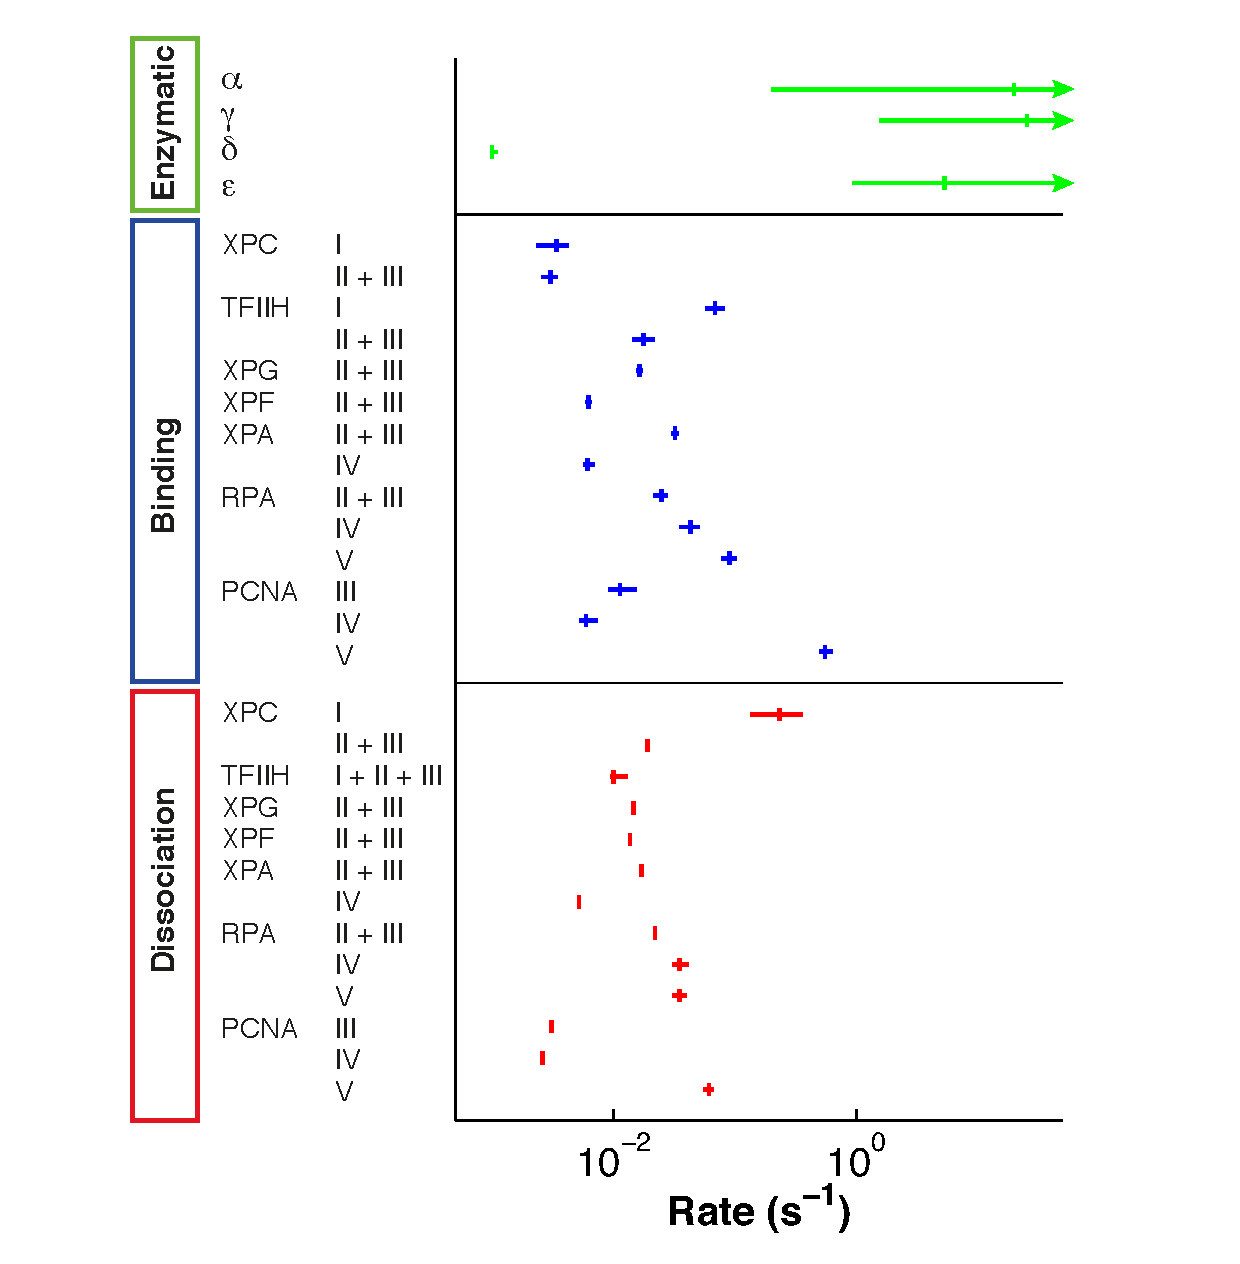
\includegraphics[width=1\textwidth]{Abbildungen/figure2_9.pdf}
		\caption{\textbf{Parameterization identifies realistic model of NER.} Mean values (vertical bars) and confidence intervals (horizontal bars) of catalytic (green), binding (blue) and dissociation constants (red) characterizing the dynamic assembly of NER factors at the successive repair intermediates (damaged DNA I, unwound DNA II, incised DNA III, resynthesized DNA IV, rechromatinized DNA V). Arrow heads indicate infinite confidence intervals.}
		\label{fig:PLE_NER_overview}
	\end{center}
\end{figure}

\begin{landscape}
	\centering
\begin{table}[t]
	\begin{adjustwidth}{}{}
	\small{
	\begin{tabular}[angle=90]{p{2cm}ccccccc}
	\hline
	\textbf{Value}    & \textbf{ XPC} & \textbf{TFIIH} & \textbf{XPG} & \textbf{XPF} & \textbf{XPA} & \textbf{RPA} & \textbf{PCNA}  \\
	\hline
	\multicolumn{8}{l}{\textbf{Damaged DNA}} \\
	$\text{K}_{\text{d}}$({\textmu}$\text{M})$                                                  & 9.35                & 0.052 & NA &NA&NA&NA&NA     \\
	& (3.46;16.09)     &(0.044;0.072)  &&&&&   \\
	\multicolumn{8}{l}{\textbf{Unwound DNA}} \\
	$\text{K}_{\text{d}}$({\textmu}$\text{M})$                                                  & 0.864                     & 0.204                   & 0.395                 &2.446                 &0.147                    &1.222                    &NA     \\
	& (0.635;1.006)     & (0.163;0.259)             & (0.373;0.419)		&(2.344; 2.596)&(0.138;0.158)     &  (1.048;1.36)  &   \\
	\multicolumn{8}{l}{\textbf{Incised DNA}} \\
	$\text{K}_{\text{d}}$({\textmu}$\text{M})$                                                  & 0.864                     & 0.204                   & 0.395                 &2.446                 &0.147                    &1.222                    &0.388     \\
	& (0.635;1.006)     & (0.163;0.259)             & (0.373;0.419)		&(2.344; 2.596)&(0.138;0.158)     &  (1.048;1.36) 	 & (0.319;0.538)  \\
	\multicolumn{8}{l}{\textbf{Resynthesized DNA}} \\
	$\text{K}_{\text{d}}$({\textmu}$\text{M})$                                                  & NA                          &NA                         & NA                      &NA                      &0.236                   &1.167                    &0.605     \\
	&                               &                              &                           &                          &(0.222;0.27)     &  (0.924;1.521)  & (0.531;0.747)  \\
	\multicolumn{8}{l}{\textbf{Rechromatinized DNA}} \\
	$\text{K}_{\text{d}}$({\textmu}$\text{M})$                                                  & NA                          &NA                         & NA                      &NA                      &NA                         &0.538                    &0.154     \\
	&                               &                              &                           &                          &                            &  (0.438;0.645)  & (0.134;0.182)  \\
	\hline
\end{tabular}}
\captionsetup{width=1.24\textwidth}
\caption{\textbf{$\text{K}_{\text{d}}$Values.} NA, not applicable. $K_d$ ($k_{\text{off}}/k_{\text{on}}$) values are given for every repair protein and arranged in columns. Reference parameter set and 95\% confidence intervals (in parentheses) are shown.}\label{tab:KdValues}
\end{adjustwidth}
\end{table}

\end{landscape}

The narrow confidence bounds on the parameters allow us to make valid computational predictions. For example, we can simulate the so far not observable fraction of incised DNA (cf.\ Figure \ref{fig:ModelFit_intermed}, green trajectory). As the EdU incorporation measurement shows, the damaged (blue) and repaired DNA (red) kinetics are tightly coupled and thereby omitting a higher accumulation of incised DNA. 

\begin{figure}[htbp]
	\begin{center}
		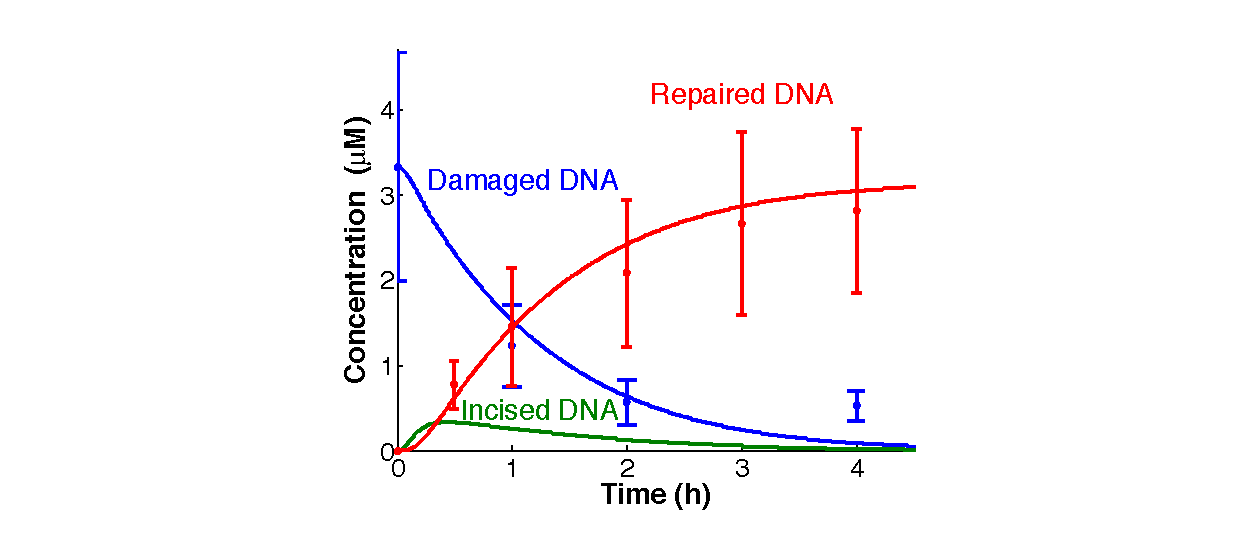
\includegraphics[width=1\textwidth]{Abbildungen/figure2_7.pdf}
		\caption{\textbf{Short delay between DNA damage removal and DNA repair synthesis omits accumulation of incised DNA.} Experimental (dots with error bars) and simulated (lines) time courses for damaged DNA (blue) and DNA repair synthesis (red). Simulated trajectories depict repair intermediate I+II for damaged DNA and repair intermediate IV+V for repaired DNA (cd.\ Figure \ref{fig:ModelStructure}). Estimated errors are depicted as shaded area. Model prediction for incised DNA (green) constitutes from DNA repair intermediate III. }
		\label{fig:ModelFit_intermed}
	\end{center}
\end{figure}


  